\documentclass[titlepage, a4paper, 10pt]{article}

\usepackage{amssymb}
\usepackage{amsmath}
\usepackage{pgfplots}
\usepackage[margin=1in]{geometry}
\usepackage{fancyhdr}
\usepackage{xcolor}
\usepackage{array}
\usepackage{bm}
\usepackage{tikz}
\usepackage{booktabs}
%\usetikzlibrary{mindmap}

\title{\normalsize PLUS Session Worksheet \\[1em] \Large \textit{MATH 1554:} Linear Algebra}
\date{Fall 2023}
\author{\textit{Covering sections}: 2.8 -- 2.9}

% ------- Set up header -------
\renewcommand{\sectionmark}[1]{\markright{#1}} % from https://tex.stackexchange.com/a/317393/227665
\pagestyle{fancy}
\fancyhead[L]{Fall 2023}
\fancyhead[C]{\textit{\nouppercase{\rightmark}}}
\fancyhead[R]{\textbf{\thepage}}
% -------------------------------------------------------

% ------- Set up math stuff -------
\renewcommand{\vec}[1]{\bm{#1}}
\DeclareMathOperator{\vspan}{Span}
\DeclareMathOperator{\row}{row}
\DeclareMathOperator{\col}{col}
\DeclareMathOperator{\colspace}{Col}
\DeclareMathOperator{\nullspace}{Nul}
\DeclareMathOperator{\rank}{rank}
% -------------------------------------------------------

% ------- Set up Main Idea box environment -------
\newcounter{mainideas}
\setcounter{mainideas}{1}
\newcommand{\mainidea}{\textbf{Main Idea \#\themainideas \stepcounter{mainideas}}}
\setlength\fboxsep{1em}
%\newcommand{\midea}[2]{\begin{center}\fbox{\parbox{#1}{\centering \mainidea #2}} \end{center}} % Could be environment but I couldn't bother

% The way this works is that the savebox collects whatever was between the minipage and the end of it, then in the last line of the definition of the environment
% we regurgigate whatever was collected into an fbox which we center.
\newsavebox{\mybox}
\newenvironment{mideea}[1]
{%
\begin{lrbox}{\mybox}%
	\begin{minipage}{#1\textwidth}
		{\centering \mainidea \par}

}
{\end{minipage}\end{lrbox}\begin{center}\fbox{\usebox{\mybox}}\end{center}}
% -------------------------------------------------------

% ------- Set up activity environment -------
\newcounter{question}
\setcounter{question}{1}
\newenvironment{newquestion}
{
	\noindent\textbf{Question \thequestion}
}
{
\stepcounter{question}
\par
}
% -------------------------------------------------------

% ------- Set up circle -------
\newcommand{\bubble}{\tikz[baseline=-0.625ex]\draw[radius=0.5em, fill=white] (0,0) circle;}
\newcommand{\dbubble}{\tikz[baseline=-0.625ex]\draw[radius=0.5em, fill=black] (0,0) circle;}
% -------------------------------------------------------

\begin{document}
\maketitle

\section{\centering T/F Questions}
\begin{newquestion} Mark each statement as \emph{true} if it's always true, or \emph{false} otherwise.
	\begin{table}[!h]
		\centering
		\begin{tabular}{c@{\hspace{2.5em}}cp{0.8\textwidth}}
			true & false & \\
			\specialrule{\lightrulewidth}{0.25em}{1.25em}
		         \bubble & \bubble & Every line in \(\mathbb{R}^n\) a subspace.\\[0.75em]
			 \bubble & \bubble & If \(A \vec{x} = A \vec{y} = \vec{b}\), for some \(A \in \mathbb{R}^{m \times n}\) and 
						       \(\vec{x}, \vec{y} \in \mathbb{R}^{n}\), then \(2\vec{x} - 2\vec{y} \in \nullspace A\).\\[0.75em]
			\bubble & \bubble & The zero vector is part of any basis of a subspace of \(\mathbb{R}^n\). \\[0.75em]
			\bubble & \bubble & Given a \(m \times n\) matrix \(A\) such that for all vectors \(\vec{x}, \vec{y} \in \mathbb{R}^n\), 
						      \(A\vec{x} = A\vec{y}\), then \(\nullspace A = \mathbb{R}^n\).\\[1.75em]
			\bubble & \bubble & Given any \(m \times n\) matrix \(A\) and it's echelon form \(U\), \(\colspace A = \colspace U\).\\[0.75em]
			\bubble & \bubble & Given any \(m \times n\) matrix \(A\) and it's echelon form \(U\), \(\nullspace A = \nullspace U\).\\[0.75em]
			\bubble & \bubble & If \(A\) is \(n \times n\) and \(\rank A = n\), then \(\nullspace A\) is empty.\\[0.75em]
			\bubble & \bubble & If \(\vec{v}\) lives in a 2-dimensional subspace of \(\mathbb{R}^3\), then it's coordinate under a basis for the subspace 
						      has 2 entries.\\[1.75em]
		\bottomrule
		\end{tabular}
	\end{table}
\end{newquestion}

\section{\centering Possible/Impossible Questions}
\begin{newquestion} If the statement \emph{could} be true, mark it as \emph{possible}. Otherwise, mark it as \emph{impossible}.
	\begin{table}[!h]
		\centering
		\begin{tabular}{c@{\hspace{2.5em}}cp{0.7\textwidth}}
			possible & impossible & \\
			\specialrule{\lightrulewidth}{0.25em}{1.25em}
			\bubble & \bubble & A matrix whose columns do not form a basis for its column space. \\[0.75em]
			\bubble & \bubble & A 3-dimensional subpsace \(H\) of \(\mathbb{R}^4\), where the number of vectors in a basis for \(H\) is 2.\\[1.75em]
			\bubble & \bubble & A vector living in 2-dimensional subspace of \(\mathbb{R}^6\), but there are only 2 entries for its coordinate vector.\\[1.75em]
			\bubble & \bubble & An invertible \(n \times n\) with the dimension of the column space being less than \(n\). \\[1.75em]
			\bubble & \bubble & The nullspace of a \(3 \times 2\) matrix that has 2 pivots has a dimension of 0. \\[0.75em]
			\bottomrule 
		\end{tabular}
	\end{table}
\end{newquestion}

\section{\centering Sketching \& Short Answer Questions}
	\begin{newquestion}
		Given the sketch, determine \([\vec{x}]_\mathcal{B}\), where 
		\(\mathcal{B} = \left\{\begin{bmatrix}1 \\ 0\end{bmatrix}, \begin{bmatrix}1 \\ 1\end{bmatrix}\right\}\).
		\begin{figure}[!h]
			\centering
			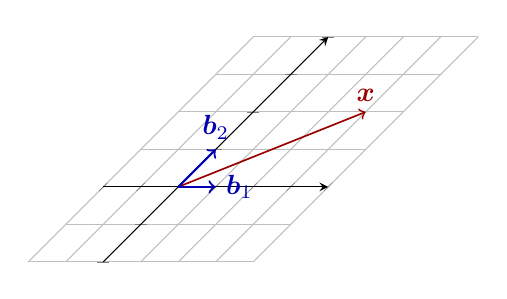
\begin{tikzpicture}
				\begin{axis}[
						anchor=center, axis lines=center, xmin=-2,xmax=4,ymin=-2,ymax=4, xtick distance=1, ytick distance=1, grid=major, 
						x={(0.75cm, 0cm)}, y={(0.75cm, 0.75cm)}, scale = 0.635, xticklabel = \empty, yticklabel=\empty]
						\addplot[->, semithick, red!60!black] coordinates {(0, 0) (3, 2)} node[above] {\(\vec{x}\)};
						\addplot[->, thick, blue!70!black] coordinates {(0, 0) (1, 0)} node[right] {\(\vec{b}_1\)};
						\addplot[->, thick, blue!70!black] coordinates {(0, 0) (0, 1)} node[above] {\(\vec{b}_2\)};
				\end{axis}
			\end{tikzpicture}
		\end{figure}
		Then, determine what \(\vec{x}\) is.
	\end{newquestion}

	\begin{newquestion}
		Find a basis for the column space and null space of the matrix \(\begin{bmatrix}1 & 6 & 4 \\ 1 & 3 & 0\end{bmatrix}\).
	\end{newquestion}

	\section{\centering Solutions}

\subsection{Solutions to T/F Questions}
	\begin{table}[!h]
		\centering
		\begin{tabular}{c@{\hspace{2.5em}}cp{0.8\textwidth}}
			true & false & \\
			\specialrule{\lightrulewidth}{0.25em}{1.25em}
		         \bubble & \dbubble & Every line in \(\mathbb{R}^n\) a subspace.\\[0.75em]
			 \dbubble & \bubble & If \(A \vec{x} = A \vec{y} = \vec{b}\), for some \(A \in \mathbb{R}^{m \times n}\) and 
						       \(\vec{x}, \vec{y} \in \mathbb{R}^{n}\), then \(2\vec{x} - 2\vec{y} \in \nullspace A\).\\[0.75em]
			\bubble & \dbubble & The zero vector is part of any basis of a subspace of \(\mathbb{R}^n\). \\[0.75em]
			\dbubble & \bubble & Given a \(m \times n\) matrix \(A\) such that for all vectors \(\vec{x}, \vec{y} \in \mathbb{R}^n\), 
						      \(A\vec{x} = A\vec{y}\), then \(\nullspace A = \mathbb{R}^n\).\\[1.75em]
			\bubble & \dbubble & Given any \(m \times n\) matrix \(A\) and it's echelon form \(U\), \(\colspace A = \colspace U\).\\[0.75em]
			\dbubble & \bubble & Given any \(m \times n\) matrix \(A\) and it's echelon form \(U\), \(\nullspace A = \nullspace U\).\\[0.75em]
			\bubble & \dbubble & If \(A\) is \(n \times n\) and \(\rank A = n\), then \(\nullspace A\) is empty.\\[0.75em]
			\dbubble & \bubble & If \(\vec{v}\) lives in a 2-dimensional subspace of \(\mathbb{R}^3\), then it's coordinate under a basis for the subspace 
						      has 2 entries.\\[1.75em]
		\bottomrule
		\end{tabular}
	\end{table}

\subsection{Solutions to Possible/Impossible Questions}
	\begin{table}[!h]
		\centering
		\begin{tabular}{c@{\hspace{2.5em}}cp{0.7\textwidth}}
			possible & impossible & \\
			\specialrule{\lightrulewidth}{0.25em}{1.25em}
			\dbubble & \bubble & A matrix whose columns do not form a basis for its column space. \\[0.75em]
			\bubble & \dbubble & A 3-dimensional subpsace \(H\) of \(\mathbb{R}^4\), where the number of vectors in a basis for \(H\) is 2.\\[1.75em]
			\dbubble & \bubble & A vector living in 2-dimensional subspace of \(\mathbb{R}^6\), but there are only 2 entries for its coordinate vector.\\[1.75em]
			\bubble & \dbubble & An invertible \(n \times n\) with the dimension of the column space being less than \(n\). \\[1.75em]
			\dbubble & \bubble & The nullspace of a \(3 \times 2\) matrix that has 2 pivots has a dimension of 0. \\[0.75em]
			\bottomrule 
		\end{tabular}
	\end{table}

\subsection{Solutions to Short Answer Questions}
	\begin{enumerate}
		\item \([\vec{x}]_\mathcal{B} = \begin{bmatrix}3 \\ 2\end{bmatrix}\). \(\vec{x} = \begin{bmatrix}5 \\ 2\end{bmatrix}\).
		\item \[\begin{bmatrix}1 & 6 & 4 \\ 1 & 3 & 0\end{bmatrix} \sim \begin{bmatrix}1 & 6 & 4 \\ 0 & -3 & -4\end{bmatrix}.\] 
			Since there's a pivot in the first two columns, the first two columns of \(\begin{bmatrix}1 & 6 & 4 \\ 1 & 3 & 0\end{bmatrix}\), 
			\(\left\{\begin{bmatrix}1 \\ 0\end{bmatrix}, \begin{bmatrix}6 \\ 3\end{bmatrix}\right\}\) form \emph{a} basis for 
			\(\colspace \begin{bmatrix}1 & 6 & 4 \\ 1 & 3 & 0\end{bmatrix}\).
		
			Continuing off, 
			\[\begin{bmatrix}1 & 6 & 4 \\ 0 & -3 & -4\end{bmatrix} \sim \begin{bmatrix}1 & 0 & -4 \\ 0 & -3 & -4\end{bmatrix}
			  \sim \begin{bmatrix}1 & 0 & -4 \\ 0 & 1 & 4/3\end{bmatrix}\]
			This corresponds to the system
			 \begin{align*}
				      x_1 &        - 4x_3       = 0 \implies x_1 = 4x_3 \\
				      x_2 &+\frac{4}{3}x_3 = 0 \implies x_2 = -\frac{4}{3}x_3
			\end{align*}
			So 
			\[\vec{x} = \begin{bmatrix}x_1 \\ x_2 \\ x_3\end{bmatrix} = \begin{bmatrix}4x_3 \\ -4/3x_3 \\ x_3\end{bmatrix} 
				      = x_3\begin{bmatrix}4 \\ -4/3 \\ 1\end{bmatrix}.\]
			Notice what this is saying. It's saying that every \(\vec{x} \in \nullspace\biggl(\begin{bmatrix}1 & 6 & 4 \\ 1 & 3 & 0\end{bmatrix}\biggr)\) is a
			scalar multiple of \(\begin{bmatrix}4 \\ -4/3 \\ 1\end{bmatrix}\). That means that \(\begin{bmatrix}4 \\ -4/3 \\ 1\end{bmatrix}\) spans the null
			space of the matrix, and since it forms a linearly independent set, it is \emph{a} basis for the nullspace of this matrix.
	
	\end{enumerate}

\end{document}